
% --------------------------------------------------------------------
% This is a simple Beamer document that uses beamerthemesigma.sty
% Reading the comments should help you create a presentation even if
% you've never used Beamer before.
% --------------------------------------------------------------------
% Set our document class to Beamer
% \documentclass[aspectratio=169]{beamer}
\documentclass[aspectratio=169, handout]{beamer}

% Some packages for nice font encodings in the final PDF
\usepackage[utf8]{inputenc}
\usepackage[T1]{fontenc}

% From Jeff E
\usepackage{algo}

\usepackage{sigmastyle}

% To insert images
\usepackage{graphicx}

% Useful packages from the AMS
\usepackage{amsmath,amssymb,amsthm}

% Package for code highlighting
\usepackage{minted}
\setminted{linenos=true, breaklines=true, breakanywhere=true, style=default}
\usemintedstyle{monokai}


\newcommand{\inst}[1]{\langle #1 \rangle}
% Set a title
\title{Turing Machines, Decidability, \& Complexity}

% The subtitle is generally where I'd expect you to put the week
% number, thus:
\subtitle{Week \texorpdfstring{7}{Lg}}
% \texorpdfstring to remove compilation warnings if you have math here

% Whoever worked on the presentation:
\author{Sam Ruggerio}

% A date, if you'd like.
\date{}

% An institute name, if you're so inclined
% \institute{University of Illinois Urbana-Champaign}

% Use the SIGma theme for this Beamer presentation
\usetheme{sigma}
% --------------------------------------------------------------------
% Begin document
\begin{document}

% This frame is just the title.
\begin{frame}
\titlepage
\end{frame}

% A frame with the table of contents.
% This frame's title is "Outline".
\begin{frame}{Outline}
  \tableofcontents
\end{frame}

% Start a section: *sections* (subsections, etc.) are what show up in the TOC.
\section{Turing Machines}
\frame{\sectionpage}
% There's a way to automate this, see:
% https://tex.stackexchange.com/questions/178800/creating-sections-each-with-title-pages-in-beamers-slides/178803
\begin{frame}{Turing Machines}

\begin{itemize}
    \item Turing Machines were conceived by Alan Turing in 1936.
    
    \item They define the fundamental basis for all models of computation.
    
    \item They aren't necessarily fast,  but tell us what we \textit{can} compute with computers. 
\end{itemize}

\end{frame}

\begin{frame}{Turing Machines}

A Turing Machine is made of a few parts: \pause
\begin{itemize}
    \item A infinitely long, 1D tape of symbols, with blanks for unused cells. \pause
    \item A state machine, which tells what the Turing Machine should do (think: DFA/NFA) \pause
    \item The Read/Write head that points to a position on the tape.
    \item The state machine has actions of what to do upon reaching a particular state (read, write, move left, move right, accept, reject) \pause
    \item Transitions between states depending on what the Turing Machine read.
\end{itemize}
\end{frame}

\begin{frame}
  \frametitle{Turing Machine}
  \begin{center}
    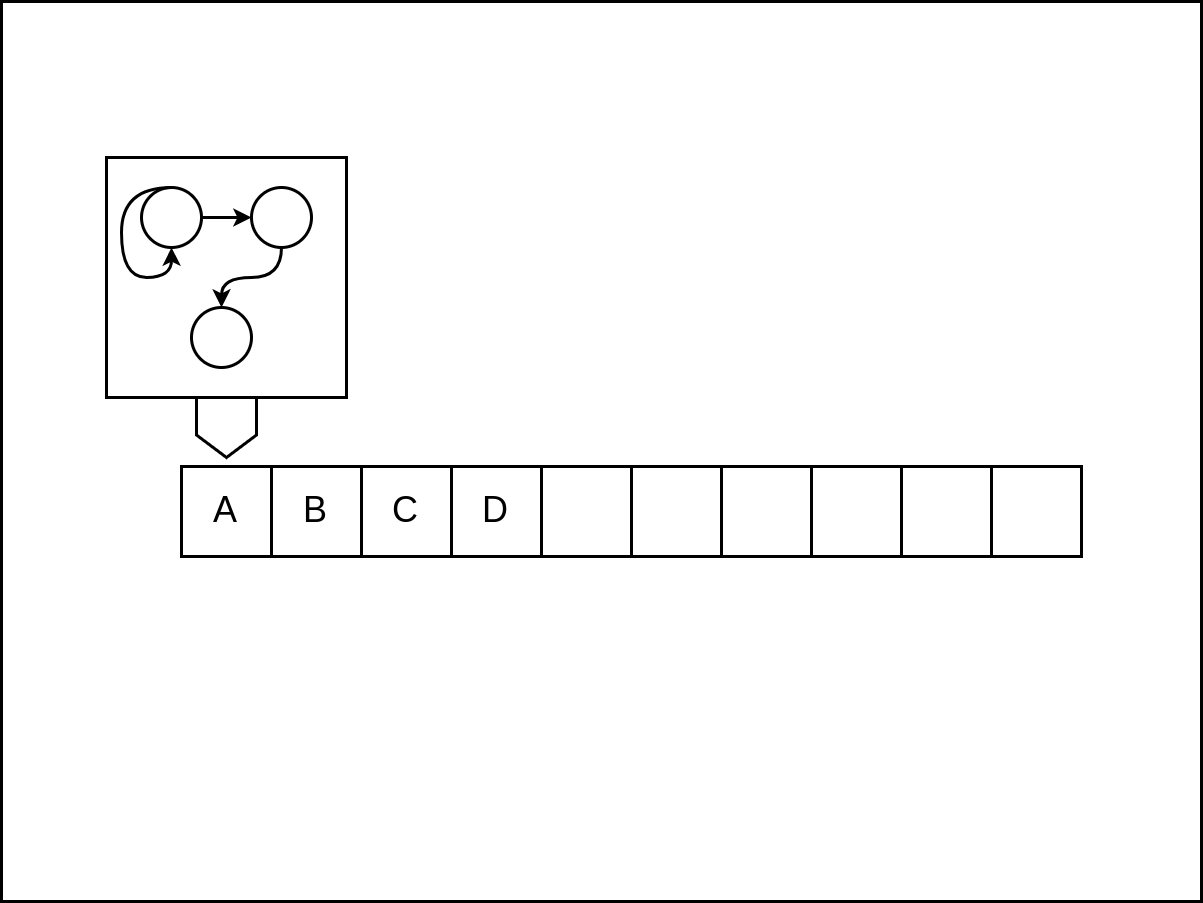
\includegraphics[width=.75\textwidth]{frame1.png}
  \end{center}
\end{frame}

\begin{frame}
  \frametitle{Turing Machine}
  \begin{center}
    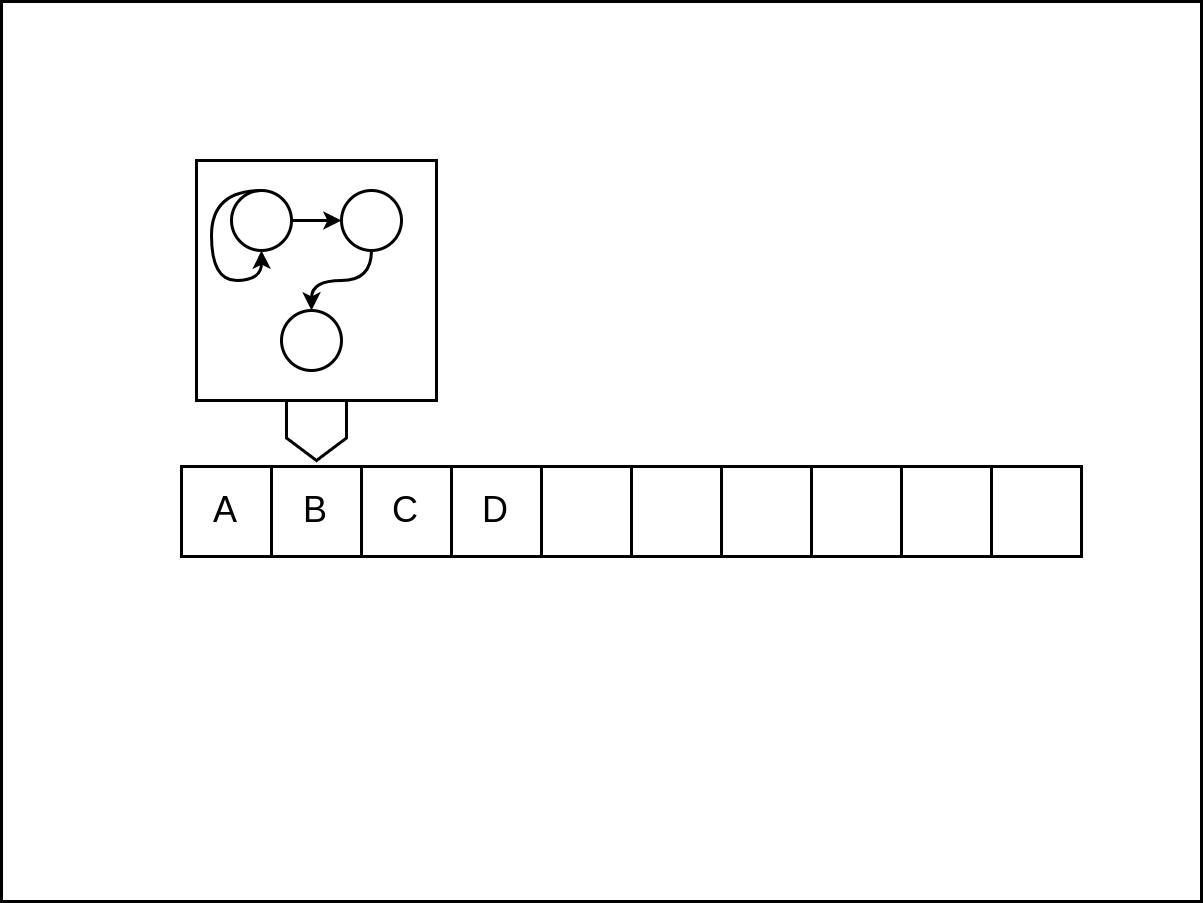
\includegraphics[width=.75\textwidth]{frame2.png}
  \end{center}
\end{frame}

\begin{frame}
  \frametitle{Turing Machine}
  \begin{center}
    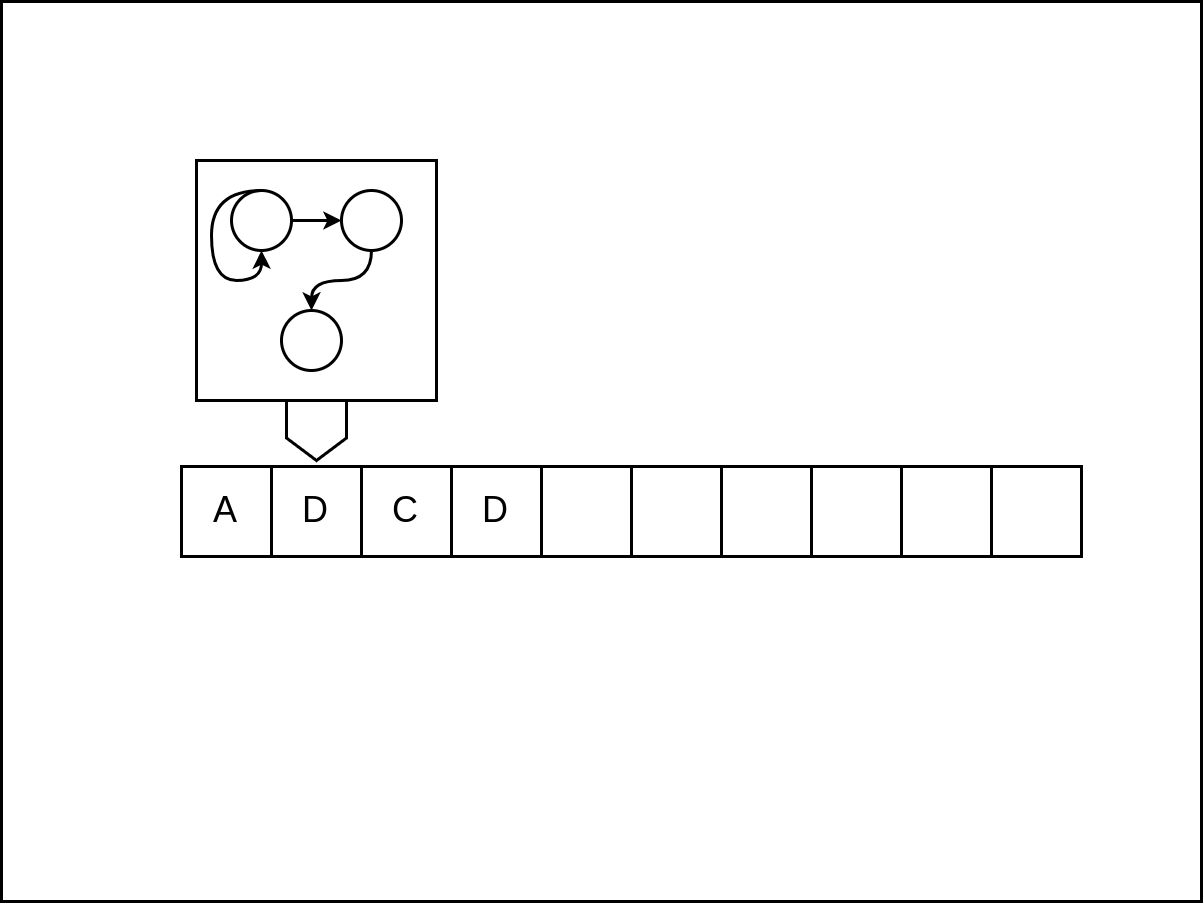
\includegraphics[width=.75\textwidth]{frame3.png}
  \end{center}
\end{frame}

\begin{frame}
  \frametitle{Turing Machine}
  \begin{center}
    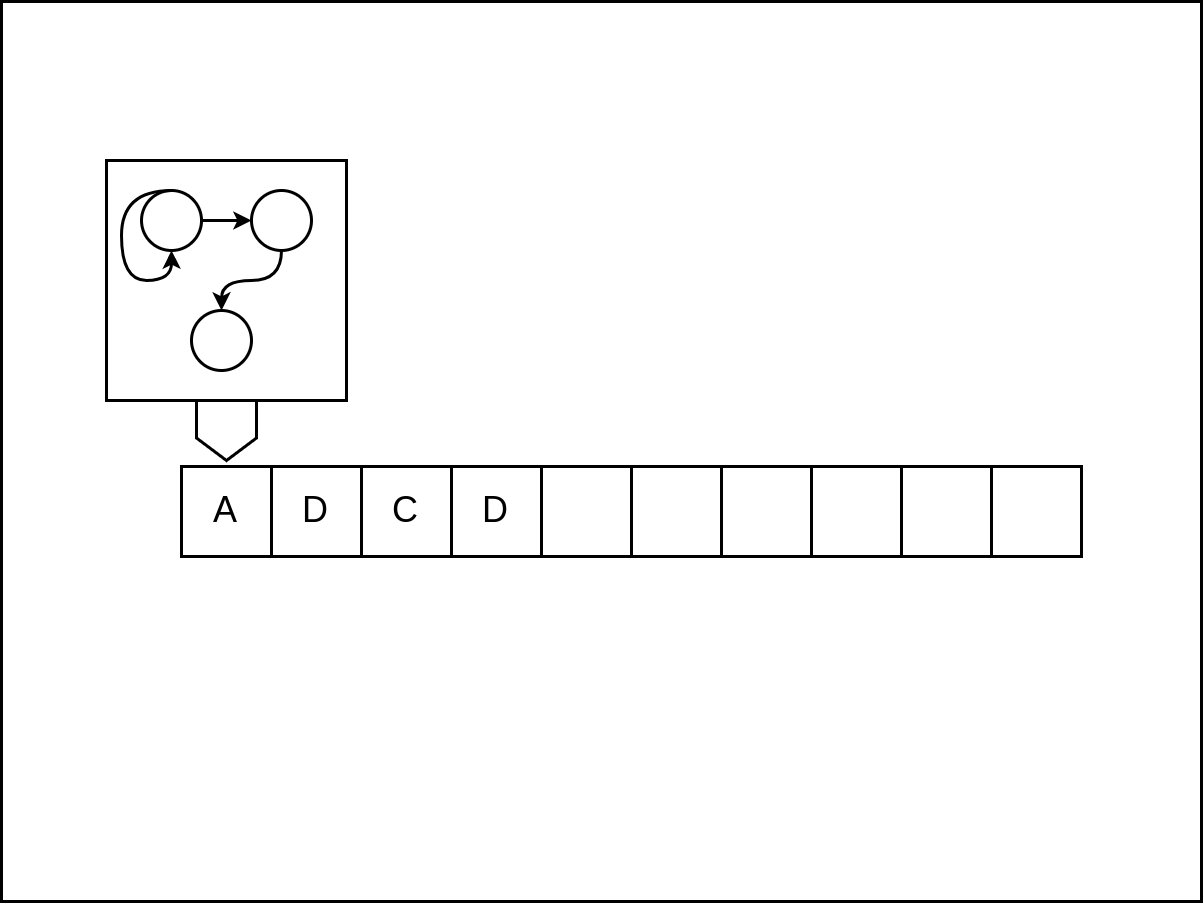
\includegraphics[width=.75\textwidth]{frame4.png}
  \end{center}
\end{frame}

\begin{frame}
  \frametitle{Turing Machine}
  \begin{center}
    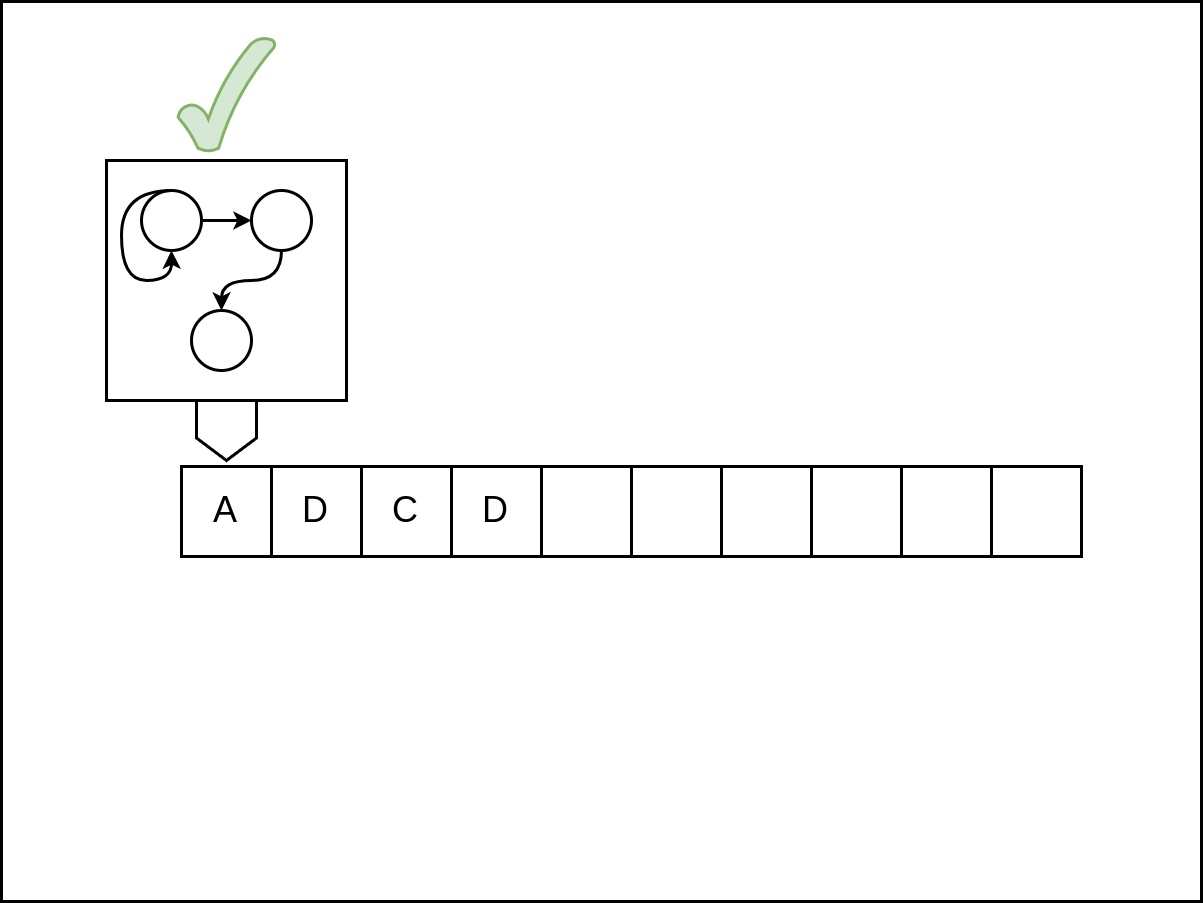
\includegraphics[width=.75\textwidth]{frame5.png}
  \end{center}
\end{frame}

\begin{frame}{Formal Definitions}
    \begin{itemize}
        \item Let the Turing Machine $M$ be defined by $(\Gamma, \Sigma, Q, \delta)$ \pause
        \item $\Gamma$ is the tape alphabet, the set of symbols that can appear on the tape. The blank symbol is included: $\epsilon \in \Gamma$ \pause
        \item $\Sigma$ is the input alphabet, the set of symbols that can \textit{initially} appear on the tape: $\Sigma \subseteq \Gamma \setminus \{\epsilon\}$ \pause
        \item $Q$ is the set of states. Three states are required to be in $Q$: \textsc{start, accept, reject}. Let $Q'$ be $Q$ without accept/reject \pause
        \item $\delta$ is the transition function: $Q' \times \Gamma \to Q \times \Gamma \times \{-1, +1\}$
    \end{itemize}
\end{frame}

\begin{frame}{Tedium}
    \begin{itemize}
        \item Turing machines are as fundamental as you can get w.r.t computation. \pause
        \item As such, the programs are very long and complex for simple problems. \pause
        \item Alonzo Church and Turing effectively proved that any problem that can be decided, can be decided with a Turing Machine (Church-Turing Thesis).
    \end{itemize}
\end{frame}

\begin{frame}{}
    \begin{center}
        {\color{sigma@mainblue} \LARGE Questions?}
    \end{center}
\end{frame}

\section{Decision Problems}
\frame{\sectionpage}

\begin{frame}{Decision Problems}
    Decision problems are strictly true and false queries:

    \begin{center}
    "What is \textbf{the index} of an element less than $k$?" 
    
    vs.
    
    "\textbf{Does this} array contain a value less than $k$?"
    \end{center}
\end{frame}

\begin{frame}{Decision Problems}
Given an \textbf{oracle}, \textsc{SmallestIDecision}, which tells you whether an array has an element less than $k$, we can figure out which index that value is stored:
    \begin{center}
    \begin{algo}
    \underline{\textsc{SmallestI}$(A[1..n],k)$}:\+
    \\ \emph{ind} $\gets 0$
    \\ for $i \gets 1$ to $n+1$:\+
    \\    if \textsc{SmallestIDecision}$(A[i..n],k) = \textsc{False}$:\+
    \\        \emph{ind} $\gets i-1$
    \\        break\-\-
    \\ return \emph{ind}
    \end{algo}
    \end{center}
\end{frame}

\begin{frame}{Questions!}
Try solving \textit{using} the decision problem, \textit{without} comparing characters.
Specifically, you should only solve these by checking if something equals \textsc{True} or \textsc{False}. (No, '1' does not typecheck to \textsc{True})
\begin{enumerate}
    \item How many 0s are in a string $w$?
    
    Does the string $w$ have $k$ 0s: \textsc{DecisionKZero}$(w, k)$ 
    
    \item How many pairs of 1s are in a string $w$?
    
    Is the number of $1s$ in a string $w$ even?  \textsc{Decision1Even}$(w)$ 
\end{enumerate}
\end{frame}

\begin{frame}{Questions!}
    \begin{algo}
    \underline{\textsc{CountZeros}$(w[1..n])$}:\+
    \\ for $k \gets 1$ to $n$:\+
    \\    if \textsc{DecisionKZero}$(w,k) = \textsc{True}$:\+
    \\          return $k$
    \end{algo}
    
    \begin{algo}
    \underline{\textsc{Count1Pairs}$(w[1..n])$}:\+
    \\ $c \gets 0$
    \\ for $i \gets 1$ to $n$:\+
    \\    if \textsc{Decision1Even}$(w[i]) = \textsc{False}$:\+
    \\          $c \gets c + 0.5$\-\-
    \\  return $\lfloor c \rfloor$
    \end{algo}
\end{frame}


\begin{frame}{Decision Languages}
    If a problem only has a true or false response, we can define a language of that problem:
    
    $$\textsc{SAT} = \{w \in \Sigma^* \mid w \text{ is a satisfiable boolean formula}\}$$
    $$\textsc{SORT} = \{w \in \Sigma^* \mid w \text{ defines a sorted integer array}\}$$
    $$\textsc{HALT} =  \{w \in \Sigma^* \mid w \text{ is a program that halts}\}$$
\end{frame}

\begin{frame}{Turing Machines \& Problems}
For any Turing machine $M$ and language $L$:
    \begin{itemize}
        \item We say that $M$ \textbf{\textit{recognizes/accepts}} $L$ if for any input $w\in L$, $M$ accepts $w$. \pause
        \begin{itemize}
            \item It's fine for $M$ to never stop on inputs that aren't in $L$, but it must accept every element of $L$. \pause
        \end{itemize}
        \item $M$ \textbf{\textit{decides}} $L$ if for any input $w$, $M$ accepts if $w \in L$ and rejects otherwise.
    \end{itemize}
\end{frame}

\begin{frame}{Turing Machines \& Languages}
For any Turing machine $M$ and input $w$:
    \begin{itemize}
        \item \textsc{Accept($M$)}: the language of all inputs $w$ where $M$ accepts. \pause
        \item \textsc{Reject($M$)}: the language of all inputs $w$ where $M$ rejects. \pause
        \item \textsc{Halt($M$)}: the language of all inputs $w$ where $M$ gives a response (halts). \pause
        \item \textsc{Diverge($M$)}: the language of all inputs $w$ where $M$ never halts.
    \end{itemize}
\end{frame}

\begin{frame}{Code is Data}
\begin{itemize}
    \item We can represent a Turing machine as a string encoding. (Enumerate the states, what state to go to, map the symbols to binary, etc.) \pause
    
    \item The input to a Turing machine can be a Turing machine itself! (Think: programs running programs/VMs/Compilers/etc.) \pause
    
    \item We use $M$ to say "the Turing Machine $M$", and $\inst{M}$ to say "the encoding of Turing Machine $M$"
\end{itemize}
\end{frame}

\begin{frame}{Simulating Machines}
\begin{itemize}
    \item Assume we have a Turing Machine $U$ designed to simulate another Turing machine $M$ on a given input $w$. \pause
    \item This instance is denoted like so: $\inst{M, w}$ \pause
    \item The language of machines that accept their input is defined as:
    $$ \textsc{ACCEPT} = \{\inst{M, w} \mid M \ \text{accepts}\ w\} $$
\end{itemize}
\end{frame}

\begin{frame}{Halting Problem}
    \begin{itemize}
        \item We cannot decide (accepting/rejecting all inputs) whether a Turing program will halt.
        \item This result was proven by Turing in his original paper. \pause
        \item Walkthrough of this proof in a future meeting!
    \end{itemize}
\end{frame}

\begin{frame}{}
    \begin{center}
        {\color{sigma@mainblue} \LARGE Questions?}
    \end{center}
\end{frame}

\begin{frame}{Questions!}
Sanity Check:
\begin{enumerate}
    \item Is the language following language \textbf{recognizable} by a Turing Machine: $\textsc{HALT} = \{ \inst{M, w} | M \text{ halts on input } w\}$ 
    \item Can $\inst{M}$ be an input to Turing Machine $M$?
    \item Can $M$ decide what will happen with itself? (i.e. $\inst{M,\inst{M}}$)
\end{enumerate}
\end{frame}

\section{Complexity}
\frame{\sectionpage}

\begin{frame}{Runtime}
    Turing machines give us metrics to measure algorithm runtime. If given an input of length $n$: \pause
    \begin{enumerate}
        \item How many steps does the Turing Machine take until it halts? (Runtime) \pause
        \item How many cells on the tape does the Turing Machine use? (Space)
    \end{enumerate}
\end{frame}

\begin{frame}{Complexity Classes}
    \begin{itemize}
        \item Define $\textsc{P}$ to be the set of decision \textit{problems} that are decidable in polynomial time. \pause
        \item Define $\textsc{NP}$ to be the set of decision problems that are decidable in polynomial time via non-determinism. \pause
        \item Define $\textsc{EXP}$ to be the set of decision problems that are decidable in exponential time. \pause
        \item Define $\textsc{NEXP}$ to be the set of decision problems that are decidable in exponential time via non-determinism.
    \end{itemize}
\end{frame}

\begin{frame}{Complexity Classes}
    What's above \textsc{NEXP}? \pause
    \begin{itemize}
        \item Define $R$ to be the set of decision problems that are decidable. \pause
        \item Define $RE$ to be the set of decision problems that are recursively  enumerable/recognizable. (Halts, if the answer is Yes).
    \end{itemize}
\end{frame}

\begin{frame}{Complexity Classes}
    What about space? \pause
    \begin{itemize}
        \item Define \textsc{PSPACE} to be the set of decision problems that are decidable in polynomial space. \pause
        \item Define \textsc{EXPSPACE} to be the set of decision problems that are decidable in exponential space.
    \end{itemize}
\end{frame}

\begin{frame}{Relations}
    We know that \textsc{P} and \textsc{NP} are subsets of \textsc{PSPACE}, but are any of these sets equal? \pause
    
    Is \textsc{PSPACE} = \textsc{EXPTIME}? \pause

    Is \textsc{EXPTIME} = \textsc{NEXPTIME} = \textsc{EXPSPACE}?
\end{frame}

\begin{frame}
  \frametitle{Complexity Subsets}
  \begin{center}
    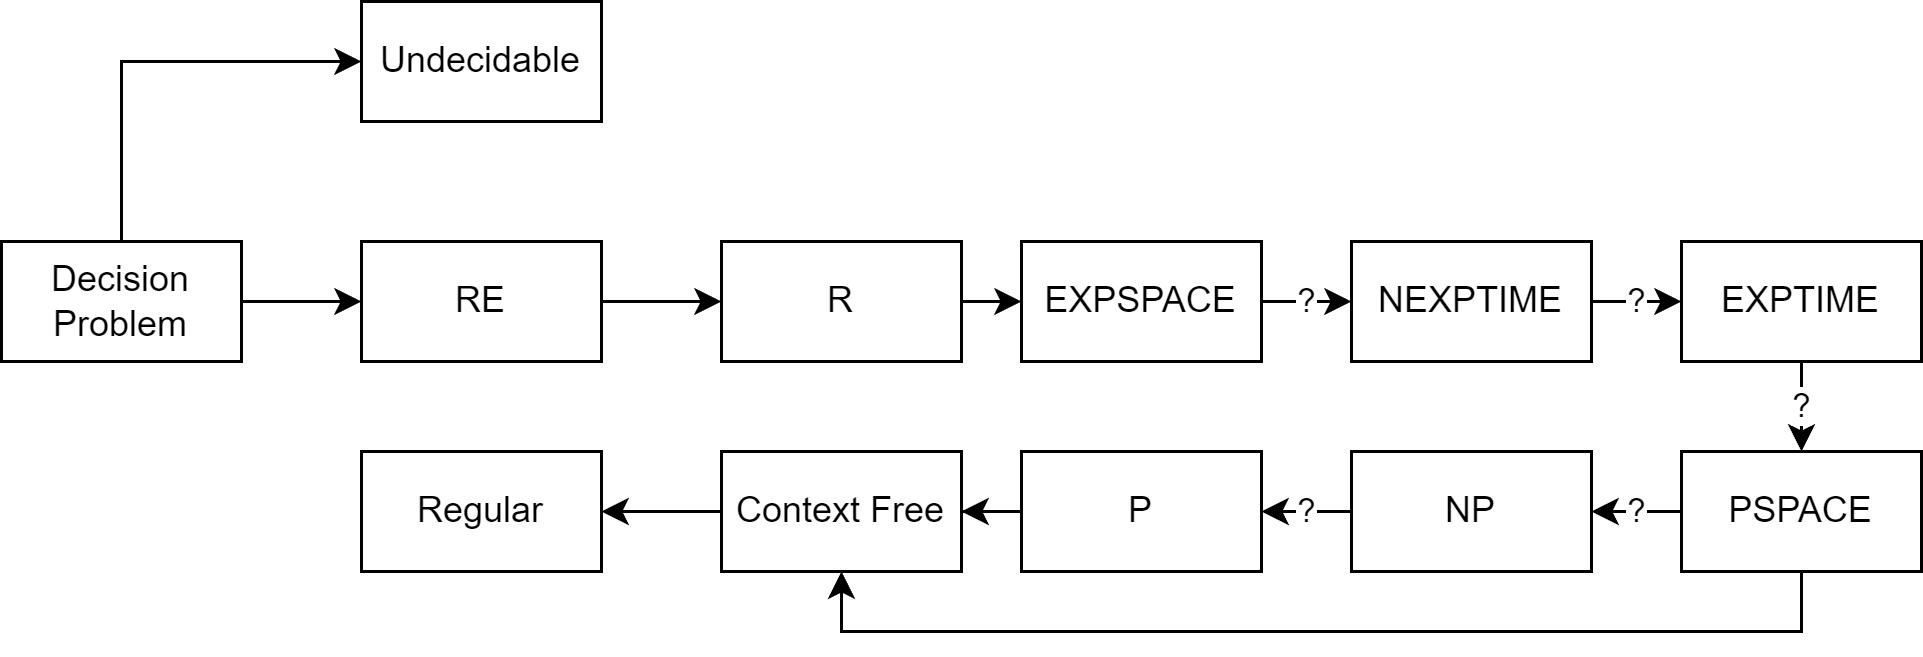
\includegraphics[width=\textwidth]{complexity.png}
  \end{center}
\end{frame}

\begin{frame}{}
    \begin{center}
        {\color{sigma@mainblue} \LARGE Questions?}
    \end{center}
\end{frame}

\end{document}